\documentclass[11pt,a4paper]{article}
\usepackage[utf8]{inputenc}
\usepackage[T1]{fontenc}
\usepackage{amsmath}
\usepackage{amssymb}
\usepackage{graphicx}
\usepackage[english]{babel}
\usepackage{lipsum}
\usepackage[scale=.75]{geometry}
\usepackage{sans}


\usepackage{fancyhdr}
\pagestyle{fancy}
\fancyhead{}
\fancyfoot{}
\renewcommand{\headrulewidth}{0pt}
\fancyfoot[R]{\thepage}



\usepackage{tikz}
\usetikzlibrary{shapes,arrows}

\tikzstyle{block} = [draw, rectangle,minimum height=1cm, minimum width=1.5cm]
\tikzstyle{sum} = [draw, circle, node distance=2cm]
\tikzstyle{input} = [coordinate]
\tikzstyle{output} = [coordinate]
\tikzstyle{gain} = [draw, isosceles triangle, minimum height=.5cm, minimum width=.5cm]
\tikzstyle{pinstyle} = [pin edge={to-,thin,black}]

\usepackage{enumitem}
\usepackage{fontawesome5}

\usepackage{listings}
\definecolor{codegreen}{rgb}{0,0.6,0}
\definecolor{codegray}{rgb}{0.5,0.5,0.5}
\definecolor{codepurple}{rgb}{0.58,0,0.82}
\definecolor{backcolour}{rgb}{0.95,0.95,0.92}
\lstdefinestyle{mystyle}{
	backgroundcolor=\color{backcolour},   
	commentstyle=\color{codegreen},
	keywordstyle=\color{magenta},
	numberstyle=\tiny\color{codegray},
	stringstyle=\color{codepurple},
	basicstyle=\ttfamily\footnotesize,
	breakatwhitespace=false,         
	breaklines=true,                 
	captionpos=b,                    
	keepspaces=true,                 
	numbers=left,                    
	numbersep=5pt,                  
	showspaces=false,                
	showstringspaces=false,
	showtabs=false,                  
	tabsize=2
}
\lstset{style=mystyle,xleftmargin=\parindent}

\usepackage{hyperref}
\hypersetup{
	colorlinks=true,
	linkcolor=black,
	filecolor=black,      
	urlcolor=blue,
	citecolor=cyan,
}

\usepackage{listings}
\definecolor{codegreen}{rgb}{0,0.6,0}
\definecolor{codegray}{rgb}{0.5,0.5,0.5}
\definecolor{codepurple}{rgb}{0.58,0,0.82}
\definecolor{backcolour}{rgb}{0.95,0.95,0.92}

\lstdefinestyle{mystyle}{
	backgroundcolor=\color{backcolour},   
	commentstyle=\color{codegreen},
	keywordstyle=\color{magenta},
	numberstyle=\tiny\color{codegray},
	stringstyle=\color{codepurple},
	basicstyle=\ttfamily\footnotesize,
	breakatwhitespace=false,         
	breaklines=true,                 
	captionpos=b,                    
	keepspaces=true,                 
	numbers=left,                    
	numbersep=5pt,                  
	showspaces=false,                
	showstringspaces=false,
	showtabs=false,                  
	tabsize=2
}

\lstset{xleftmargin=\parindent}

\usepackage{acro}

\usepackage{enumitem}

\usepackage{caption}
\captionsetup{labelfont=bf, font=footnotesize} % Bold "Figure X.Y" and reduce the caption size


% list of acronyms
\DeclareAcronym{cpp}{
	short = CPP,
	long = Coverage Path Planning,
}

\DeclareAcronym{uav}{
	short = UAV,
	long = Unmanned Aerial Vehicle,
}

\DeclareAcronym{gcs}{
	short = GCS,
	long = Ground Control Station,
}

\DeclareAcronym{qgc}{
	short = QGC,
	long = QGroundControl,
}

\DeclareAcronym{ros}{
	short = ROS,
	long = Robot Operating System,
}

\DeclareAcronym{sitl}{
	short = SITL,
	long = Software-In-The-Loop,
}

\DeclareAcronym{wsl}{
	short = WSL,
	long = Windows Subsystem for Linux,
}

\DeclareAcronym{tsp}{
	short = TSP,
	long = Travelling Salesman Problem,
}




\begin{document}
	
	\begin{titlepage}
	
	
	\begin{center}
		
		
\includegraphics[scale=.1]{unipg-logo-title-2364x1862.png} 
		
		   	
		
		\vspace{1cm}
		
		
		\vspace{.5cm}
		\textbf{\LARGE{Development and testing of methods for drones control}}
		
		\vspace{1cm}
		
		
		%\textbf{Prof. Francesco Ferrante} \\
		%{\small \href{mailto:francesco.ferrante@unipg.it}{francesco.ferrante@unipg.it}}
		%
		%\hfill
		%
		%\textbf{Dott. Mirko Leomanni} \\
		%{\small \href{mailto:mirko.leomanni@unipg.it}{mirko.leomanni@unipg.it}}
		%
		%\hfill
		
		\textbf{Paolo Leopardi}\\ \href{mailto:paolo.leopardi96@gmail.com}{paolo.leopardi96@gmail.com}
		\vspace{1cm}
		
		\begin{flushright}
			{\small Last update: \today}
		\end{flushright}
		\vspace{-.5cm}
		\rule{\textwidth}{.1cm}
		
	\end{center}
	
	\tableofcontents
	
	
\end{titlepage}
	
	\printacronyms
	
	\clearpage
	
	\section{Introduction}

The project is officially called (italian) \textit{Sviluppo e sperimentazione di metodologie di controllo per droni} and it lies in the field of agricultural robots. The aim of these months will be the implementation of a real drone which is able to move in a area and take informations autonomously through some device mounted on the robot (thermal imager). The project can be splitted in two main parallel directions:
\begin{itemize}
	\item Navigation (path planner, control schemes, etc.)
	\item Implementation (drone construction, autopilot selection, etc.)
\end{itemize}

	\section{Navigation}
To successfully cover the area of interest the quadcopter has to navigate following a certain logic and take into account different factors such as the shape and the dimension of the area, presence of obstacles, vehicle used and so on. There is a class of algorithm called \ac{cpp} which is well suited for this aim.

\subsection{Coverage Path Planning}
Given an area of interest the \ac{cpp} problem consist of planning a path which covers the entire target environment considering the vehicle's motion restriction and sensor's characteristics, while avoiding passing over obstacles \cite{cabreira2019survey}. These algorithms can be classified into two main categories: offline and online \cite{fevgas2022coverage}. Offline algorithms need a previous knowledge of the search area, online algorithm instead are based on real-time data acquisition.

Another classification is based on the decomposition method thaat can be classified in:
\begin{itemize}
	\item Cellular decomposition
	\begin{itemize}
		\item Exact decomposition
		\item Approximate decomposition
	\end{itemize}
	\item No decomposition
\end{itemize}
Cellular decomposition methods are based in dividing the surface into cells: in the exact decomposition the workspace is splitted in sub-areas whose re-union exactly occuped the target area \cite{cabreira2019survey}. In the approximate decomposition the area is usally divided using a grid where the size of the squares is typically determined for example by the footprint of the camera mounted on the robot. In no decomposition techniques, as the name suggest, isn't applied any type of decomposition.
Taking in to account the aim of the project, i.e. the \ac{uav} has to collect data in different positions of an area, the best solution is the approximate decomposition technique beacuse we don't need to cover every centimetre of the area (like an autonomous lawn mower), we need to determine the amount of waypoints that guarantees an exhaustive data collection compared to the target area.
	\section{Implementation}
The implementation step is the physical construction of the \ac{uav}, this involves the selection of all the elements, both hardware (e.g. platform and its components) and software (e.g. autopilot flight stack).

\subsection{Autopilot selection}
Autopilot selection is made by evaluating possible pros and cons which every autopilot fligh stack brings with it. Three possible solution were evaluated:
\begin{enumerate}
	\item INAV \cite{inav}
	\item PX4 \cite{px4}
	\item Agilicious \cite{foehn2022agilicious}
\end{enumerate}
There are a lot of reason which can determine the choice of one solution instead of another, a preliminary evaluation is made considering the informations available on the web (official documentation and other sources). These parameters have been accounted:
\begin{itemize}
	\item configuration
	\item missions definition
	\item future developments
\end{itemize}
\textit{Configuration} denotes the level of complexity needed to configure flight controller for the first flight, \textit{missions definition} takes into account how to define missions, and \textit{future development} indicates compatibility with other framework, software and so on.

INAV's configuration seems easy as PX4, the main difference is the guide: for INAV you can follow some videos on Youtube at this \href{https://www.youtube.com/playlist?list=PLOUQ8o2_nCLkfcKsWobDLtBNIBzwlwRC8}{link}, for PX4 it's necessary to follow sections from \href{https://docs.px4.io/main/en/assembly/}{\textit{Basic Assembly}} to \href{https://docs.px4.io/main/en/flying/}{\textit{Flying}} in the official documentation.
Agilicious doesn't have a section related to the configuration steps for the first real flight like the above mentioned.

INAV provide a \ac{gcs} which is capable of define only waypoints which the \ac{uav} has to visit, as shown for example \href{https://www.youtube.com/watch?v=J6UBai-OIYQ}{here}. PX4 typically use \ac{qgc} as \ac{gcs}\footnote{\ac{qgc} supports only PX4 and Ardupilot}, here different missions can be defined and it is worth to note that there is also survey missions which seems particularly suited with the aim of this project. Agilicious doesn't not provide a \ac{gcs} for missions definition, but it has a module called \href{https://agilicious.readthedocs.io/en/main/modules/references.html}{\texttt{reference}} which implements different ways of generating reference trajectories.

I wasn't able to find any documentation regarding interfacing between INAV and \ac{ros}, PX4 has a subsection dedicated to \href{https://docs.px4.io/main/en/ros/}{ROS communication with PX4}. In addiction PX4 has a MATLAB package called UAV Toolbox Support Package for PX4 Autopilots \cite{mathworkspx4}. 
Agilicious has a very good structure for future developments beacause you can change controller or estimator by simply modify a \texttt{yaml} file. It's not provided a way to integrate GPS measurements. An interface  for \ac{ros} called \href{https://agilicious.readthedocs.io/en/main/integration/ros.html}{\texttt{agiros}} is provided. Both PX4 and Agilicious docs propose a simulator.  

In conclusion the better idea should be to try the autopilot in this order: PX4, Agilicious, INAV.

%todo vedi se inserire una sezione con le varie componenti hardware utilizzate

\subsection{PX4 configuration}
Before first flight PX4 Autopilot needs some steps to follow to configure the autopilot, this one are documented in PX4 documentation's section called \href{https://docs.px4.io/main/en/config/}{Standard Configuration}. The procedure is quite straightforward but some problems may arise during these steps.

\subsection*{Troubleshooting}
\begin{description}[style=nextline]
	\item[Firmware version] \ac{qgc} provides au automatic way to flash the latest firmware\footnote{At the time of writing this report, i.e. September 2023, the last stable release is \texttt{v1.13.3}.}, however all version 13 express same problem with our specific hardware. More specifically the problem is related to the Wi-Fi module because with the firmware version \texttt{v1.13.x} the autopilot is unable to connect with \ac{qgc}. So I found that version \texttt{v1.12.3}\footnote{Firmware releases available \href{https://github.com/PX4/PX4-Autopilot/releases}{here}.} fixes this problem.
	\item [Autotune] Having downgraded to the version \texttt{v1.12.3} determined the impossibility to use the autotune procedure because this is available from \texttt{v1.13.0}.
\end{description}

%todo da qualche parte prova a scrivere anche del problema del magnetometro

\subsection{Optitrack configuration}
After some outside experiments (in which human pilot successfully drove the quadcopter) we decided to take the next flight test in an indoor scenario; this beacause an indoor environment is safer if compared to the outdoor one in terms of damaged caused by the drone's crashing.

Before flying, the communication between Optitrack and flight controller needs to be configured, we can think the Optritrack as the indoor counterpart of the GPS. To configure the Optritrack with PX4 there also a dedicated section named \href{https://docs.px4.io/main/en/ros/external_position_estimation.html}{Using Vision or Motion Capture Systems for Position Estimation}, this one provides all the necessary steps to configure the communication. Please note that there is also a \href{https://docs.px4.io/main/en/ros/external_position_estimation.html#specific-system-setups}{dedicated subsection} for Optitrack system.

\subsection*{Troubleshooting}
\begin{description}[style=nextline]
	\item[Parameters] Having used an older firmware version, some parameters\footnote{Full parameter list \href{https://docs.px4.io/main/en/advanced_config/parameter_reference.html}{here}.} have been replaced with others; these ones are listed in the table below. The first column shows the actual name of the parameters the second columns shows the counterpart on the firmware version used in this project.
	\begin{center} 
	\begin{tabular}{|c|c|}
		\hline
		PX4 docs naming & \texttt{v1.12.3} naming \\
		\hline
		\texttt{EKF2\_EV\_CTRL}  &  \texttt{EKF2\_AID\_MASK}  \\
		\hline
		\texttt{EKF2\_HGT\_REF}  &  \texttt{EKF2\_HGT\_MODE}   \\
		\hline
		\texttt{EKF2\_GPS\_CTRL} & \texttt{EKF2\_AID\_MASK}  \\
		\hline
	\end{tabular}
\end{center}
	Another set of parameters are the ones used for the preflight check, Disabling these prevents the drone from checking the correct operation of the corresponding sensors:
	\begin{itemize}
		\item \texttt{SYS\_HAS\_BARO}
		\item \texttt{SYS\_HAS\_GPS}
		\item \texttt{SYS\_HAS\_MAG}
		\end{itemize}
	
	 

\end{description}

	\section{Simulation}
To test some \ac{cpp} algorithms is worth to implement an environment which allows to drive a drone autonomously in a safe way, without any risk of collision. PX4 offers different simulators which allow to develop \ac{sitl} simulation \cite{px4_simulation}. More in details, in the section named \textit{MAVROS Offboard control example (Python)} \cite{px4_ros_mavros} there is a useful example on how to setup PX4, Gazebo and MAVROS to run a simulation.

To implement a complete pipeline which allows to develop \ac{cpp} algorithms, simulate the quadcopter and analyse the result MATLAB has been employed beside the simulator structure which exploit PX4, Gazebo and MAVROS, mentioned above. MATLAB is used to determine the area, develop the \ac{cpp} algorithms and pass the waypoint to the simulator. After the simulation phase, which is executed in Gazebo environment the results are visualized and analysed in MATLAB again.

MATLAB is executed in Windows environment, while PX4 software stack, Gazebo and of course \ac{ros} are executed in \ac{wsl} environment (more specifically in Ubuntu 20.04).

\subsection{MATLAB code} 
There are two main files called \texttt{main.m} and \texttt{WSL\_connection.m}; the first one deals with the definition of the target area by the user, the execution of the \ac{cpp} algorithm and consequently the determination of waypoints in space. The second one is devoted to establish the connection with \ac{wsl} to send the waypoint calculated in the \texttt{main.m} file.
\subsubsection*{Main.m code}
As mentioned previously the \texttt{main.m} code is responsible for determining the area of interest and the waypoint calculation.
The first section allows the user to select an area by specifying the latitude and longitude as shown in \ref{fig:target_area_selection}. After the selection procedure the area is converted in local coordinate expressed in meters. This further step is needed because waypoints will be calculated based on robot's footprint.
\lstinputlisting[language=Octave, linerange={5-37}, firstnumber=5]{../simulator/main.m}
\begin{figure}[hbt!]
	\centering
	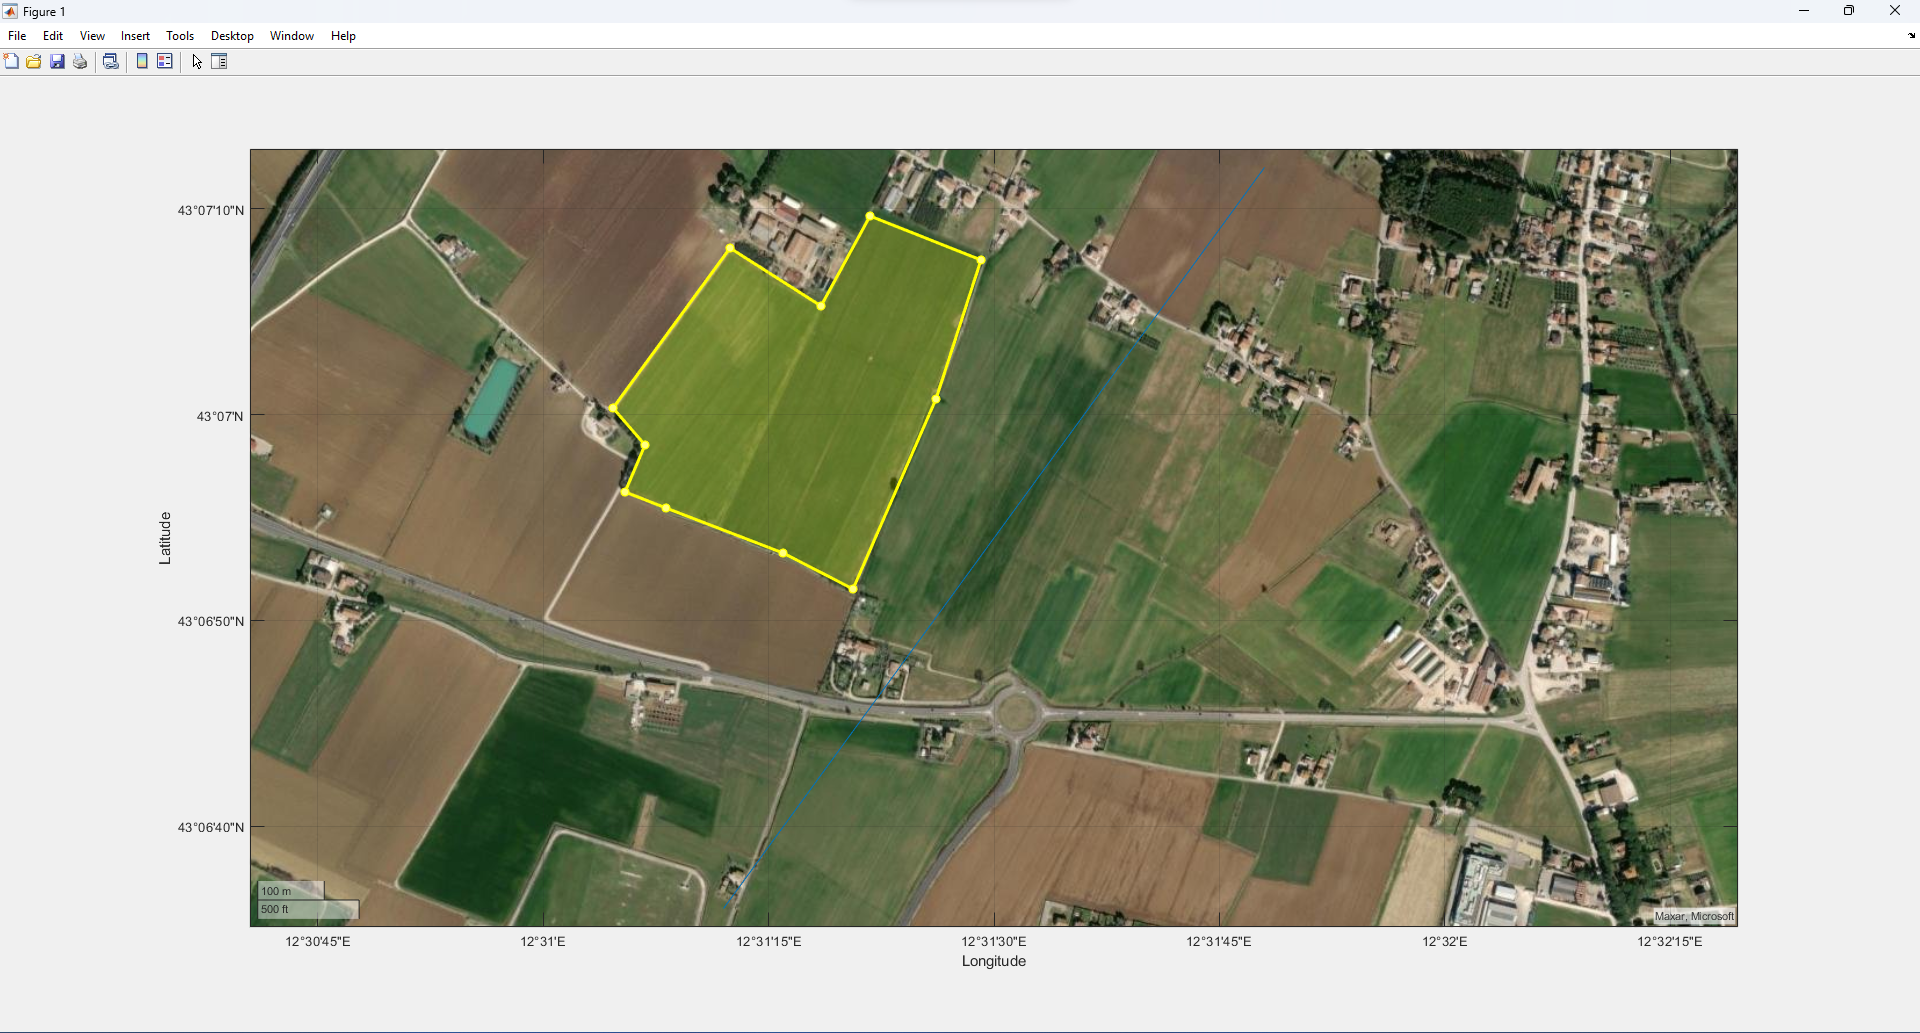
\includegraphics[width=\linewidth]{images/target_area_selection}
	\caption{Target area selection.}
	\label{fig:target_area_selection}
\end{figure}

The next section is devoted to the computation of the waypoints related to the selected area.
\lstinputlisting[language=Octave, linerange={39-71}, firstnumber=39]{../simulator/main.m}
\begin{figure}[hbt!]
	\centering
	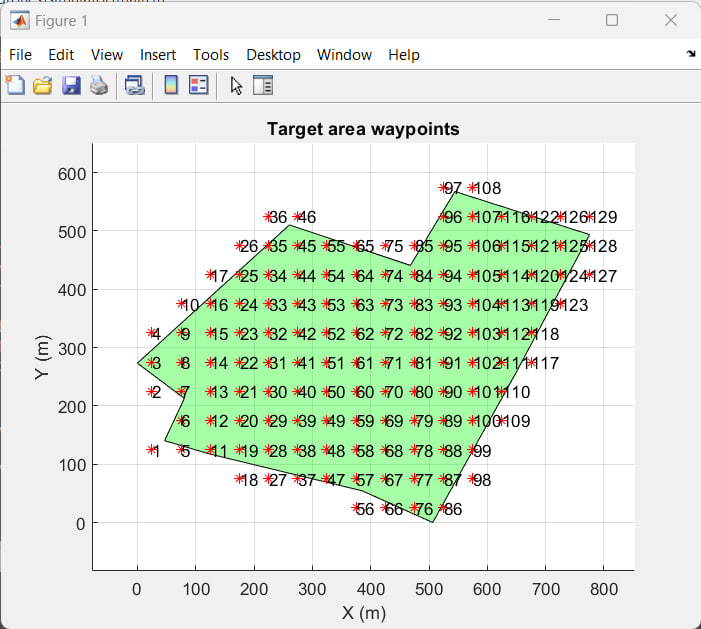
\includegraphics[width=.75\linewidth]{images/waypoints_calculation}
	\caption{Computation of waypoints.}
	%\label{fig:calculations_waypoints}
\end{figure}

The following part sorts the waypoints by applying the algorithm based on the \ac{tsp} \cite{tsp_wikipedia}. MATLAB solver for a general \ac{tsp} is available at \href{https://it.mathworks.com/help/optim/ug/traveling-salesman-problem-based.html}{\textit{Traveling Salesman Problem: Problem-Based}}, the function named \texttt{TSP\_waypoints} implement this example with minor adjustments. The variable named \texttt{waypoints\_sequence} stores the waypoints order, the variable named \texttt{waypoints\_ordered} stores the sequence of waypoints computed by the \ac{tsp} algorithm.
\lstinputlisting[language=Octave, linerange={73-89}, firstnumber=73]{../simulator/main.m}
\begin{figure}[hbt!]
	\centering
	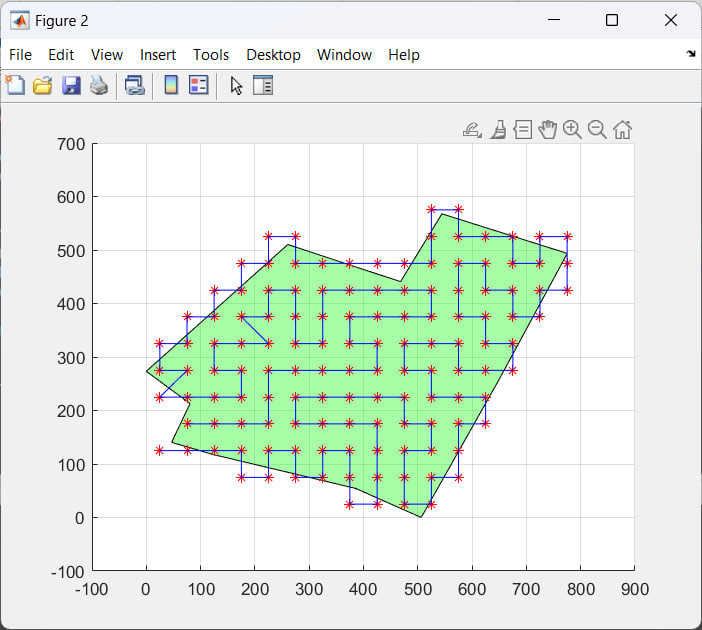
\includegraphics[width=.5\linewidth]{images/waypoints_ordered}
	\caption{Waypoints ordered by the \ac{tsp} algorithm.}
	%\label{fig:ordered_waypoints}
\end{figure}

The last section is responsible for the analysis of the data collected in the simulation. An example on how to get the trajectory of the quadcopter from rostopic is provided\footnote{Please note that the file named \texttt{rosbag\_2.bag} is only an example and so the data recorded couldn't be related with the current waypoints computed.}.

\subsection*{WSL\_connection.m code}
This script is responsible for the connection with \ac{wsl}, which means that allows MATLAB to interact with the rostopic executed on \ac{wsl}, it automatically recovers the ip addresses needed
\footnote{This code is tested in Windows system, to recover the addresses through Windows terminal and ubuntu shell type the following commands: 
\begin{itemize}
	\item In Ubuntu shell type \texttt{\$ ifconfig} and look for the address named \texttt{iner} under \texttt{eth0}. This is the variable named \texttt{ipAdd\_wsl}.
	\item In Windows terminal type \texttt{\$ ip config} and look for \texttt{IPv4 address} under \texttt{Ethernet Card vEthernet (WSL). This is the variable named \texttt{ipAdd\_Windows}}.
\end{itemize}}.
\lstinputlisting[language=Octave, linerange={1-23}, firstnumber=1]{../simulator/WSL_connection.m}

In addition, the second section is responsible of instantiating a new node which publish the waypoint list\footnote{The code assumes that there is a matrix variable named \texttt{waypoint3D}, wtih dimensions $N \times 3$, where $N$ represents the number of waypoint and the columns are the $xyz$ coordinates in the space.} in the topic named \texttt{/MATLAB\_waypoint}.
\lstinputlisting[language=Octave, linerange={26-49}, firstnumber=26]{../simulator/WSL_connection.m}

\subsection{WSL environment}
\ac{wsl} is used to run the simulations, it exploits the PX4 autopilot with Gazebo and MAVROS. First of all the following components need to be installed:
\begin{itemize}
	\item PX4 autopitlot folder, downloadable by following the section named \href{https://docs.px4.io/main/en/dev_setup/dev_env_linux_ubuntu.html}{\textit{Ubuntu Development Environment}}. 
	\item \ac{ros} and MAVROS\footnote{The installation of \ac{ros} and MAVROS is not covered in this guide.}
\end{itemize}
The idea behind the simulation is to use MAVROS to drive in off-board mode a simulated quadcopter in Gazebo using the waypoints computed in MATLAB. As a result, we need a ac{ros} that is capable of subscribing to the topic named \texttt{/MATLAB\_waypoint} to recover the waypoint list. By following PX4 documentation sections named \href{https://docs.px4.io/main/en/ros/mavros_offboard_python.html}{\textit{MAVROS Offboard control example (Python)
}} is easy to understand how to develop a new \ac{ros} package\footnote{\texttt{catkin\_make} can be used instead of\texttt{catkin build}, for more details take a look at ROS documentation section named \href{http://wiki.ros.org/ROS/Tutorials/CreatingPackage}{\textit{Creating a ROS Package}.
}}.
The file implemented to create the rosnode is called \texttt{waypoint\_manager.py}. 

\subsubsection*{Waypoint\_manager.py}
The code should be easily readable by the user, for more details contact the author. %TODO explain the code 
 % the code is written in lstlisting env beacause is not possible to link it since it lies in WSL env
\begin{lstlisting}[language=Python]
	#!/usr/bin/env python3
	
	import rospy
	from geometry_msgs.msg import PoseStamped, Point, PoseArray
	from mavros_msgs.msg import State
	from mavros_msgs.srv import CommandBool, CommandBoolRequest, SetMode, SetModeRequest
	from math import dist
	
	
	current_state = State()
	
	waypoint_index = 0
	waypointList = []
	waypointReceived = False # flag to check if waypoint list is received
	nextWaypoint = [0, 0, 0]
	
	
	
	def state_cb(msg):
		global current_state
		current_state = msg
	
	
	def buildWPArray(data):
		for index in range(len(data.poses)):
		waypointList.append([data.poses[index].position.x, data.poses[index].position.y, data.poses[index].position.z])
	
	
	def getNextWP(currentPosition, threshold):
	
		global waypoint_index
		global waypointList
		global nextWaypoint
	
		try: 
			currentWaypoint = waypointList[waypoint_index]
			nextWaypoint = currentWaypoint
			
			if dist(currentPosition, currentWaypoint) < threshold: # compute euclidean 3D distance
			waypoint_index += 1
			nextWaypoint = waypointList[waypoint_index]
			rospy.loginfo('Next waypoint: ' + str(nextWaypoint))             
	
		except IndexError:
			pass
	
	
	return nextWaypoint
	
	
	
	def WP_callback(data):
	
		if waypointReceived:
		
		targetWP = getNextWP([data.pose.position.x,
		data.pose.position.y,
		data.pose.position.z], threshold=.2)          
		
		
		
		# Create a PoseStamped message
		pose_msg = PoseStamped()
		pose_msg.header.stamp = rospy.Time.now()
		pose_msg.pose.position.x = targetWP[0]
		pose_msg.pose.position.y = targetWP[1]
		pose_msg.pose.position.z = targetWP[2]
		pose_msg.pose.orientation.x = 0.0
		pose_msg.pose.orientation.y = 0.0
		pose_msg.pose.orientation.z = 0.0
		pose_msg.pose.orientation.w = 0.0
		
		currentWaypoint_pub.publish(pose_msg)
		
		#else:
		#    rospy.loginfo('Waiting for waypoint')
	
	if __name__ == '__main__':
	
		try:
		
		rospy.init_node('waypoint_manager')
		
		# subscribers
		state_sub = rospy.Subscriber("mavros/state", State, callback = state_cb)
		position_sub = rospy.Subscriber('mavros/local_position/pose', PoseStamped, callback = WP_callback)
		
		# publisher
		currentWaypoint_pub = rospy.Publisher('/mavros/setpoint_position/local', PoseStamped, queue_size=10)
		
		
		rospy.wait_for_service("/mavros/cmd/arming")
		arming_client = rospy.ServiceProxy("mavros/cmd/arming", CommandBool) 
		
		rospy.wait_for_service("/mavros/set_mode")
		set_mode_client = rospy.ServiceProxy("mavros/set_mode", SetMode)
		
		waypointMessage = rospy.wait_for_message("/MATLAB_waypoint", PoseArray)
		buildWPArray(waypointMessage)
		rospy.loginfo("Waypoint list: " + str(waypointList))
		waypointReceived = True    
	
	
		# Setpoint publishing MUST be faster than 2Hz
		rate = rospy.Rate(20)
		
		# Wait for Flight Controller connection
		while(not rospy.is_shutdown() and not current_state.connected):
			rate.sleep()
	
		offb_set_mode = SetModeRequest()
		offb_set_mode.custom_mode = 'OFFBOARD'
	
		arm_cmd = CommandBoolRequest()
		arm_cmd.value = True
		
		last_req = rospy.Time.now()
	
		while(not rospy.is_shutdown()):
			if(current_state.mode != "OFFBOARD" and (rospy.Time.now() - last_req) > rospy.Duration(5.0)):
				if(set_mode_client.call(offb_set_mode).mode_sent == True):
					rospy.loginfo("OFFBOARD enabled")
	
				last_req = rospy.Time.now()
				
			else:
				if(not current_state.armed and (rospy.Time.now() - last_req) > rospy.Duration(5.0)):
					if(arming_client.call(arm_cmd).success == True):
						rospy.loginfo("Vehicle armed")	
						
					last_req = rospy.Time.now()
	
			rate.sleep()
	
		rospy.spin()
	
	except rospy.ROSInterruptException:
		rospy.logwarn("Node Interrupted")
\end{lstlisting}

\subsection{Execute simulation}
Is recommendable to don't use a \texttt{.launch}, launch all the files from different terminal. These are the steps to successfully run the simulation:
\begin{enumerate}
	\item Run \texttt{main.m} file to compute the waypoints
	\item On the first terminal run the command \texttt{\$ roslaunch PX4-Autopilot/launch/mavros\_posix\_sitl.launch} to launch the PX4 autopoilot and Gazebo environment
	\item On the second terminal run the command \\
	\texttt{\$ rosrun offboard\_py waypoint\_manager.py} to launch the \texttt{waypoint\_manager} node
	\item Run \texttt{WSL\_connection.m} to send the waypoint list to the \texttt{waypoint\_manager} node
\end{enumerate}
After this the situation should look like the one depicted in Figure \ref{fig:rqt_graph_view}.
\begin{figure}[hbt!]
	\centering
	\includegraphics[width=\linewidth]{"images/rqt_graph view"}
	\caption{Node and topic view focused on \texttt{waypoint\_manager} node.}
	\label{fig:rqt_graph_view}
\end{figure}

	\clearpage
	

	
	\bibliographystyle{unsrt} 

	\bibliography{bibliography} 
	


\end{document}